\begin{frame}
	\frametitle{Interaktion Vegetation und Atmosphäre}

  \begin{figure}
    \centering
    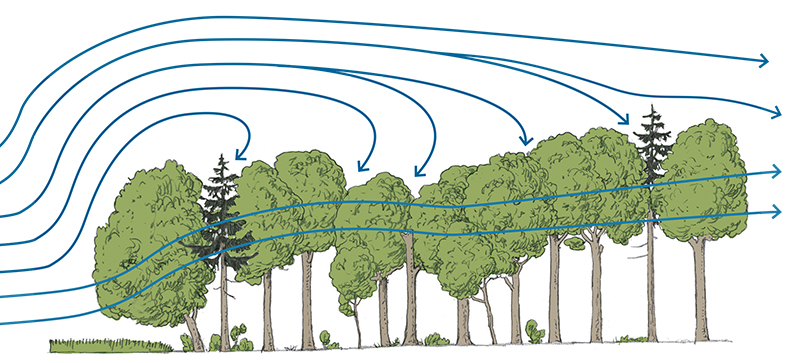
\includegraphics[width=.55\linewidth]{bilder/Wind_Vegetation.jpg}
    \caption{Wechselwirkung zwischen Atmosphäre und Biosphäre, Quelle: Stadt Kriens}
  \end{figure}
		\begin{itemize}
			\item Bodenbedeckung wirkt auf Wind, Wasseraustausch und Strahlungshaushalt
			\item [$\rightarrow$] Wälder bremsen Winde, speichern Wasser, beeinflussen Wolkenbildung und bilden Schatten und großen Lebensraum
			\item [$\rightarrow$] in Wüsten und Steppen versickert Wasser schneller und es gibt kaum Schatten, dafür existiert schwacher Albedo-Effekt
			\item Existenz und Wachstum von Vegetation bindet u.a. CO$_2$ und absorbiert Strahlung
			\item Absterben von Vegetation führt zu Freisetzung von CO$_2$ und anderen Stoffen in die Luft und Böden % Nitrat, Phosphat, Stickstoff etc.
		\end{itemize}

	\note{
		\begin{itemize}
			\item[] Photosynthese: Aufnahme von CO$_2$ und abgabe von O$_2$, Nutzung des Kohlenstoff für das Wachstum
			\item[] Lösung organischer Kohlenstoff-Verbindungen durch baterielle Zersetzung $\rightarrow$ Freisetzung von CO$_2$
			\item[] Änderungen an der Landoberfläche durch z.B: Änderung der Landnutzung - Waldrodung, Landwirtschaft ändern auch die Vegetation und die Ökosysteme
		\end{itemize}
		Fragen? Sonst $\rightarrow$ Klimamodelle
	}
\end{frame}

%\begin{frame}
%	\frametitle{Interaktion Vegetation und Atmosphäre}
%
%		\begin{figure}
%		\centering
%		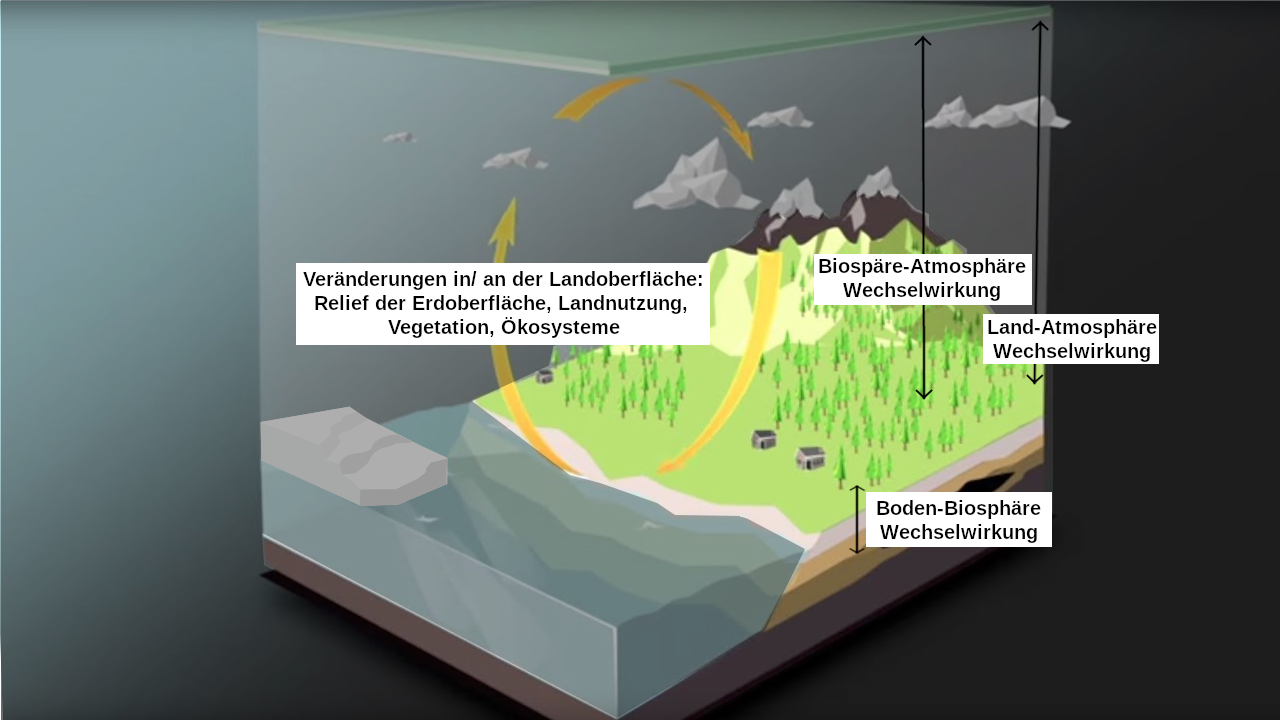
\includegraphics{bilder/WMO_Cycles_factors_landAndGround.png}
%		\caption{Interaktion der Biosphäre und Atmosphäre}
%	\end{figure}
%
%	\note{
%		\begin{itemize}
%			\item[] diesmal sind rechts die Wechselwirkungen der Vegetation und %Biosphäre zu sehen
%			\item[] links sind nochmal die zentralen Elemente der Komponente %Vegetation aufgelistet
%		\end{itemize}
%	}
%\end{frame}
